% f2015gdl_q18_solid.tex — 2015 年高考数学·广东卷·理科 第 18 题（四棱锥 P-ABCD 立体图）
%
% 【来源】`.work/phase3-b17/source/2015广东理.pdf`（SHA-256
%   1c3faab50a5d1fb2bdba424104c10910341e7362d222e018fb27e631578daa9a），
%   第 2 页（合订本页 948）第 1 栏；内容对象 21。
%
% 【坐标口径】清单坐标为「真页 pt、原点左上、y 向下」。本图取
%   X0 = 202.0221（顶点 A 的 x），Y0 = 284.7441（顶点 A 的 y_top），
%   本地坐标  (x, y) = (x_page − X0, Y0 − y_top)，即本地原点 = 顶点 A，
%   x 向右、y 向上，1 单位 = 1 TeX pt。
%   换算示例：A (202.0221,284.7441) → (0,0)；B (365.2908,284.7441) → (163.2687,0)；
%   C (389.7813,243.9270) → (187.7592,40.8171)；D (226.5127,243.9270) → (24.4906,40.8171)；
%   P (308.1470,171.9323) → (106.1249,112.8118)。
%
% 【与广东文卷 Q18 的关系】本图几何与 `2015_广东卷_文科` Q18 图相同（x 逐点相同），
%   整体在页面上比文卷版下移 10.627pt；理科版新增 E（CD 中点）、F、G 三要素与
%   P–E、G–F 两条线段。文理互证由主会话事后完成，图源照本卷源件独立实测。
%
% 【线宽/虚线】全部棱 line width = 0.3985pt；DC 短段 dash pattern =
%   on 2.98883pt off 2.98883pt，dash phase = 0pt；无填充、无 c 算子（全为 m/l 直线）。
%
% 【照源复刻的存疑项】
%   DC 自 D 起为虚线：虚线路径为「交点 → D」（源 m (240.1184,597.9630)
%   l (226.5127,597.9630) 方向照录），相位 0 起于交点。
%   源未画棱 PB，照录不补。
%   源每条棱路径起点有零长度重复 moveto，按规范不复刻。
%
% 【自验结果】见文件末尾。
%
% 元素计数：11 条路径（9 条实线棱/线段 + DC 实线 + DC 虚线）、8 个标签。
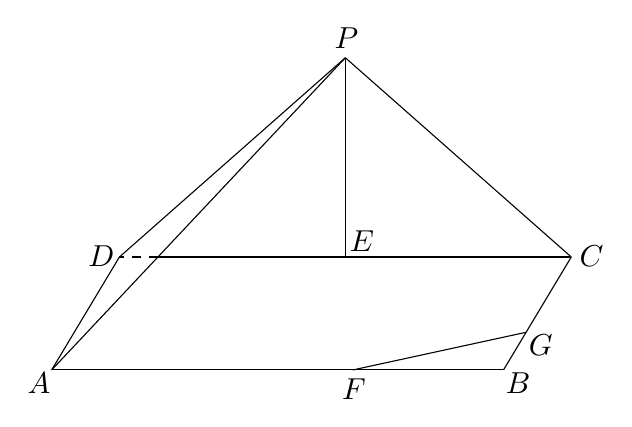
\begin{tikzpicture}[x=1pt, y=1pt,
    every node/.style={inner sep=0pt, font=\fontsize{10.5pt}{12.6pt}\selectfont}]

  % ---- 顶点（本地坐标） ----
  % A (0,0)  B (163.2687,0)  C (187.7592,40.8171)  D (24.4906,40.8171)
  % P (106.1249,112.8118)  E (106.1249,40.8171)  F (108.8458,0)  G (171.4322,13.6057)

  % ---- P–D（源 path 0：m D(226.5127,597.9630) l P(308.1470,669.9577)，本图反向） ----
  \draw[line width=0.3985pt] (106.1249,112.8118) -- (24.4906,40.8171);

  % ---- P–C（源 path 1：m P(308.1470,669.9577) l C(389.7813,597.9630)） ----
  \draw[line width=0.3985pt] (106.1249,112.8118) -- (187.7592,40.8171);

  % ---- A–D（源 path 2：m A(202.0221,557.1459) l D(226.5127,597.9630)） ----
  \draw[line width=0.3985pt] (0.0000,0.0000) -- (24.4906,40.8171);

  % ---- A–B（源 path 3：m B(365.2908,557.1459) l A(202.0221,557.1459)，本图反向） ----
  \draw[line width=0.3985pt] (0.0000,0.0000) -- (163.2687,0.0000);

  % ---- G–F（源 path 4：m G(373.4543,570.7516) l F(310.8679,557.1459)） ----
  \draw[line width=0.3985pt] (171.4322,13.6057) -- (108.8458,0.0000);

  % ---- A–P（源 path 5：m A(202.0221,557.1459) l P(308.1470,669.9577)） ----
  \draw[line width=0.3985pt] (0.0000,0.0000) -- (106.1249,112.8118);

  % ---- B–C（源 path 6：m B(365.2908,557.1459) l C(389.7813,597.9630)） ----
  \draw[line width=0.3985pt] (163.2687,0.0000) -- (187.7592,40.8171);

  % ---- P–E（源 path 7：m P(308.1470,669.9577) l E(308.1470,597.9630)） ----
  \draw[line width=0.3985pt] (106.1249,112.8118) -- (106.1249,40.8171);

  % ---- D–C 实线段（源 path 8：m C(389.7813,597.9630) l (240.1184,597.9630)） ----
  \draw[line width=0.3985pt] (187.7592,40.8171) -- (38.0963,40.8171);

  % ---- D–C 虚线段（源 path 9：m (240.1184,597.9630) l D(226.5127,597.9630)，方向照源） ----
  \draw[line width=0.3985pt, dash pattern=on 2.98883pt off 2.98883pt, dash phase=0pt]
    (38.0963,40.8171) -- (24.4906,40.8171);

  % ---- 标签：源文本 Tm 原点（基线左端），CMMI10 10.5pt ----
  \node[anchor=base west] at (102.0249,116.1981) {$P$};  % 源 (304.0470,673.3440)
  \node[anchor=base west] at (13.0239,37.2291)   {$D$};  % 源 (215.0460,594.3750)
  \node[anchor=base west] at (190.6049,37.2291)  {$C$};  % 源 (392.6270,594.3750)
  \node[anchor=base west] at (-8.8691,-8.5189)   {$A$};  % 源 (193.1530,548.6270)
  \node[anchor=base west] at (163.9539,-8.5189)  {$B$};  % 源 (365.9760,548.6270)
  \node[anchor=base west] at (107.5829,42.8651)  {$E$};  % 源 (309.6050,600.0110)
  \node[anchor=base west] at (104.7409,-10.5619) {$F$};  % 源 (306.7630,546.5840)
  \node[anchor=base west] at (172.2359,5.0871)   {$G$};  % 源 (374.2580,562.2330)

\end{tikzpicture}
%
% 【自验结果】
%   探针：latexmk -pdfxe，0 error / 0 Overfull / 0 Underfull / 0 Missing character；
%         页面 210.45 × 133.43 pt（standalone border=0）。
%   tex 反算：10 条路径 + 8 个标签全部匹配，最大残差 0.000050 pt（阈值 0.05）。
%   600dpi 墨迹：整体墨迹包围盒最大边差 0.325 pt；几何包围盒 0.065 pt；
%         标签中心最大 0.298 pt（C）。（尺度归一，已扣除 0.996277 的
%         TeX pt / PDF bp 均匀因子）
%         按页面 bp 直接比较（物理）最大 0.655 pt，来自该 0.37% 均匀缩放。
%   灵敏度：顶点 C x +0.15pt → tex 检查器报 0.1500、600dpi 几何包围盒报 0.1204；
%         标签 E y +0.15pt → tex 检查器报 0.1500、600dpi 标签中心报 0.0946；
%         G–F 线宽 +0.02pt → 等效宽度 0.9094 → 0.9517 pt（delta +0.0423）。均能报出。
